\documentclass[tikz,border=6pt]{standalone}
\usepackage[T1]{fontenc}
\usepackage[utf8]{inputenc}
\usepackage{import}
\subimport{layers/}{init.tex}
\usetikzlibrary{arrows.meta,positioning}
\definecolor{ink}{HTML}{242629}
\definecolor{muted}{HTML}{59616a}
\definecolor{panel}{HTML}{f6f6f3}
\definecolor{blue}{HTML}{dfeaf5}
\definecolor{peach}{HTML}{f7cdae}
\definecolor{green}{HTML}{a9ce91}
\definecolor{yellow}{HTML}{ffe49b}
\definecolor{purple}{HTML}{d5c5e8}
\definecolor{white}{HTML}{ffffff}
\definecolor{heat}{HTML}{e89a50}
\definecolor{offset}{HTML}{a6bdd8}
\definecolor{size}{HTML}{ddc66e}
\definecolor{yaw}{HTML}{a8c983}
\definecolor{iou}{HTML}{b6a1cd}
\begin{document}
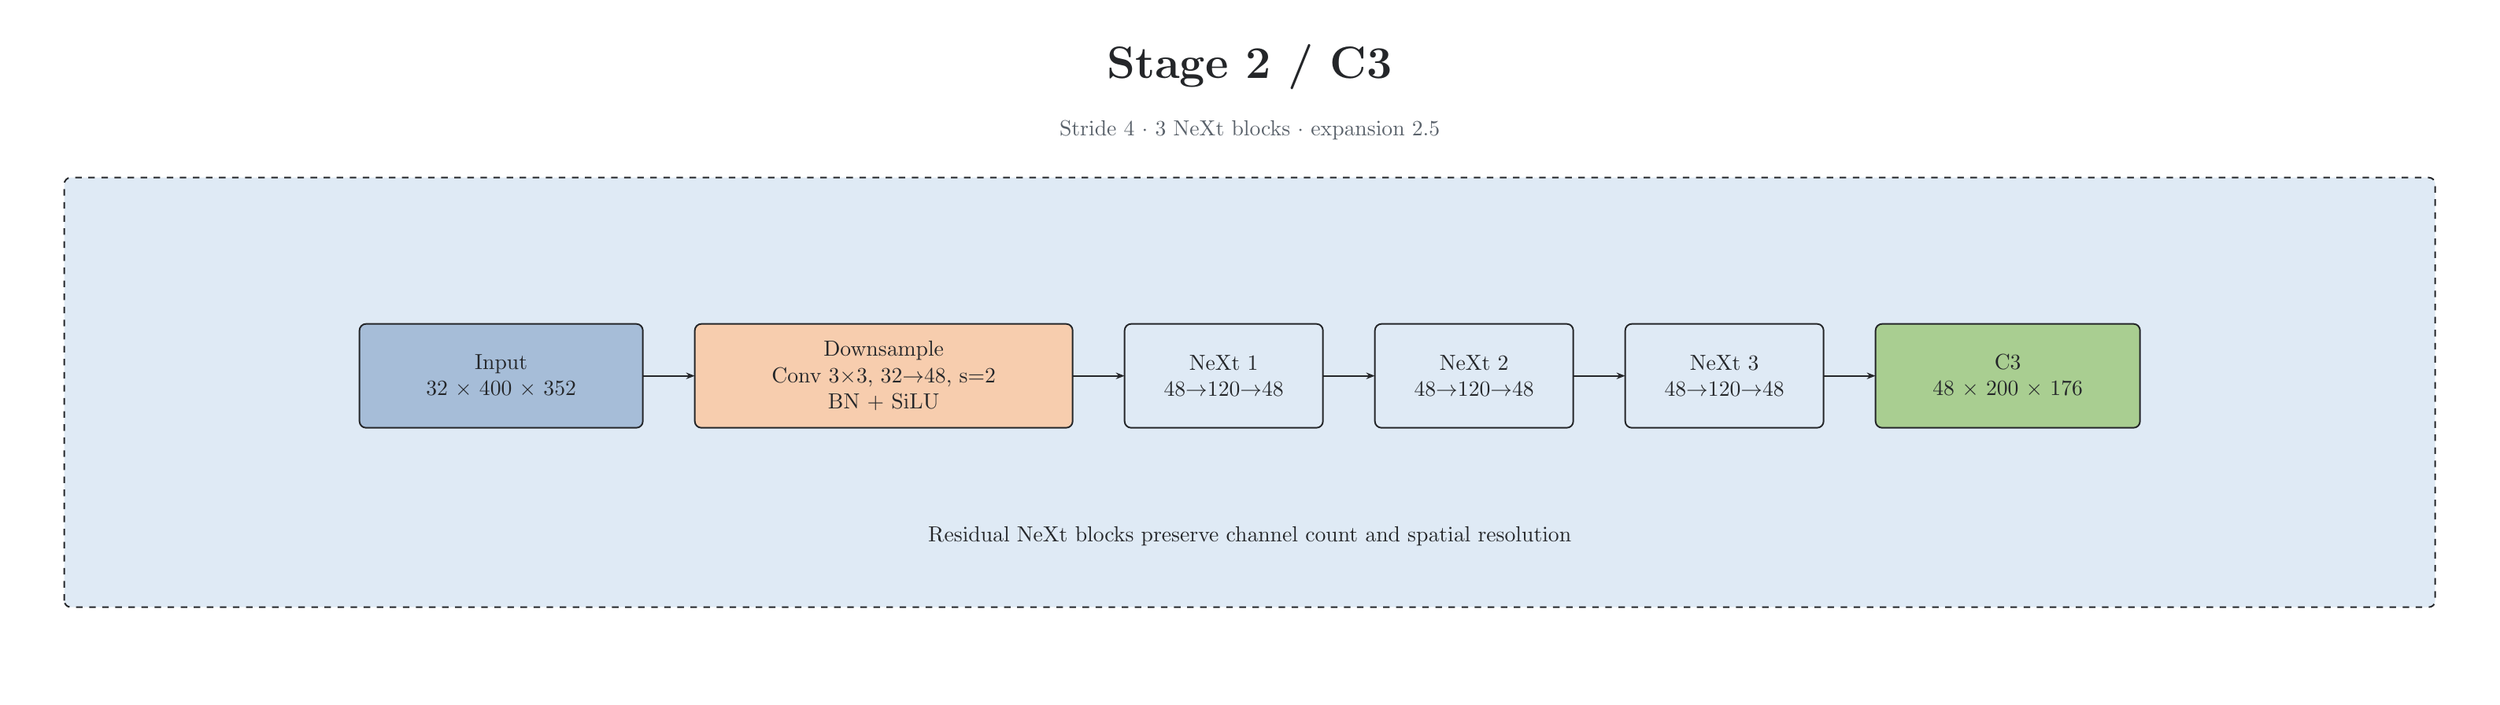
\begin{tikzpicture}[x=1.524cm,y=1.524cm,z={(0.9906cm,0.73152cm)}]
\path[use as bounding box] (0,0) rectangle (26,7);
\node[anchor=center,align=center,text=ink,font=\fontsize{20}{24.0}\selectfont \bfseries ] at (13.0,6.52) {Stage 2 / C3};
\node[anchor=center,align=center,text=muted,font=\fontsize{10}{12.0}\selectfont ] at (13.0,5.85) {Stride 4 $\cdot$ 3 NeXt blocks $\cdot$ expansion 2.5};
\draw[draw=ink,fill=blue,rounded corners=3pt,line width=.7pt,dashed] (0.4499999999999993,0.8000000000000003) rectangle (25.55,5.35);
\node[anchor=west,align=left,text=ink,font=\fontsize{15}{18.0}\selectfont \bfseries ] at (0.8,4.85) {};
\draw[draw=ink,fill=offset,rounded corners=3pt,line width=.7pt] (3.5749999999999993,2.7) rectangle (6.574999999999999,3.8);
\node[anchor=center,align=center,text=ink,font=\fontsize{10}{12.0}\selectfont ] at (5.074999999999999,3.25) {Input\\32 $\times$ 400 $\times$ 352};
\draw[-{Stealth[length=4pt]},draw=ink,line width=.7pt] (6.574999999999999,3.25) -- (7.124999999999999,3.25);
\draw[draw=ink,fill=peach,rounded corners=3pt,line width=.7pt] (7.125,2.7) rectangle (11.125,3.8);
\node[anchor=center,align=center,text=ink,font=\fontsize{10}{12.0}\selectfont ] at (9.125,3.25) {Downsample\\Conv 3$\times$3, 32$\rightarrow$48, s=2\\BN + SiLU};
\draw[-{Stealth[length=4pt]},draw=ink,line width=.7pt] (11.125,3.25) -- (11.675,3.25);
\draw[draw=ink,fill=blue,rounded corners=3pt,line width=.7pt] (11.675,2.7) rectangle (13.775000000000002,3.8);
\node[anchor=center,align=center,text=ink,font=\fontsize{10}{12.0}\selectfont ] at (12.725000000000001,3.25) {NeXt 1\\48$\rightarrow$120$\rightarrow$48};
\draw[-{Stealth[length=4pt]},draw=ink,line width=.7pt] (13.775,3.25) -- (14.325000000000001,3.25);
\draw[draw=ink,fill=blue,rounded corners=3pt,line width=.7pt] (14.325000000000001,2.7) rectangle (16.425,3.8);
\node[anchor=center,align=center,text=ink,font=\fontsize{10}{12.0}\selectfont ] at (15.375000000000002,3.25) {NeXt 2\\48$\rightarrow$120$\rightarrow$48};
\draw[-{Stealth[length=4pt]},draw=ink,line width=.7pt] (16.425,3.25) -- (16.975,3.25);
\draw[draw=ink,fill=blue,rounded corners=3pt,line width=.7pt] (16.975,2.7) rectangle (19.075000000000003,3.8);
\node[anchor=center,align=center,text=ink,font=\fontsize{10}{12.0}\selectfont ] at (18.025000000000002,3.25) {NeXt 3\\48$\rightarrow$120$\rightarrow$48};
\draw[-{Stealth[length=4pt]},draw=ink,line width=.7pt] (19.075000000000003,3.25) -- (19.625000000000004,3.25);
\draw[draw=ink,fill=green,rounded corners=3pt,line width=.7pt] (19.625000000000004,2.7) rectangle (22.425,3.8);
\node[anchor=center,align=center,text=ink,font=\fontsize{10}{12.0}\selectfont ] at (21.025000000000002,3.25) {C3\\48 $\times$ 200 $\times$ 176};
\node[anchor=center,align=center,text=ink,font=\fontsize{10}{12.0}\selectfont ] at (13,1.55) {Residual NeXt blocks preserve channel count and spatial resolution};
\end{tikzpicture}
\end{document}
